\subsection*{Информация о проекте}

Команда разработчиков из 16 человек занимается созданием карты города на
основе собственного модуля отображения. Проект должен быть завершен в
течение 6 месяцев. Бюджет проекта: 50 000 рублей.

Дата отчета: 08.05.24

Статистика:

\begin{figure}[h!]
	\begin{center}
		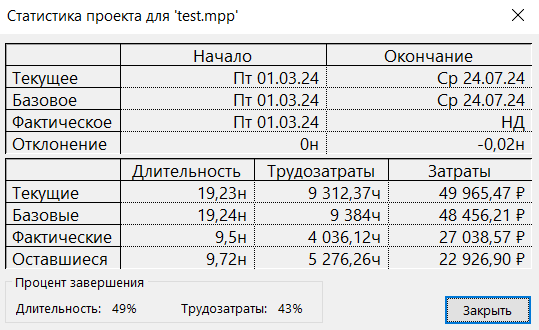
\includegraphics[scale=0.7]{inc/img/p_1.png}
	\end{center}
	\captionsetup{justification=centering}
	\label{fig:u3}
\end{figure}

\subsection*{Задание 1: работа с таблицей освоенного объёма}

\textbf{1. Проанализируйте прямые и косвенные затраты проекта на дату отчета.}

Косвенные затраты связанны с использованием ресурсов, то есть в нашем
случае это затраты на группу ресурсов Оборудование, прямые затраты,
связанные с выполнением работ – на все остальные.

Затраты на дату отчета отображены в столбце Фактические затраты, разность
между плановыми и фактическими затратами – в столбце отклонение по
стоимости.

Существеное отклонение по стоимости среди косвенных ресурсов (+5570 руб) связано с покупкой специализированного оборудования для задачи <<Создание мультимедия наполнения>>. 

\begin{figure}[h!]
	\begin{center}
		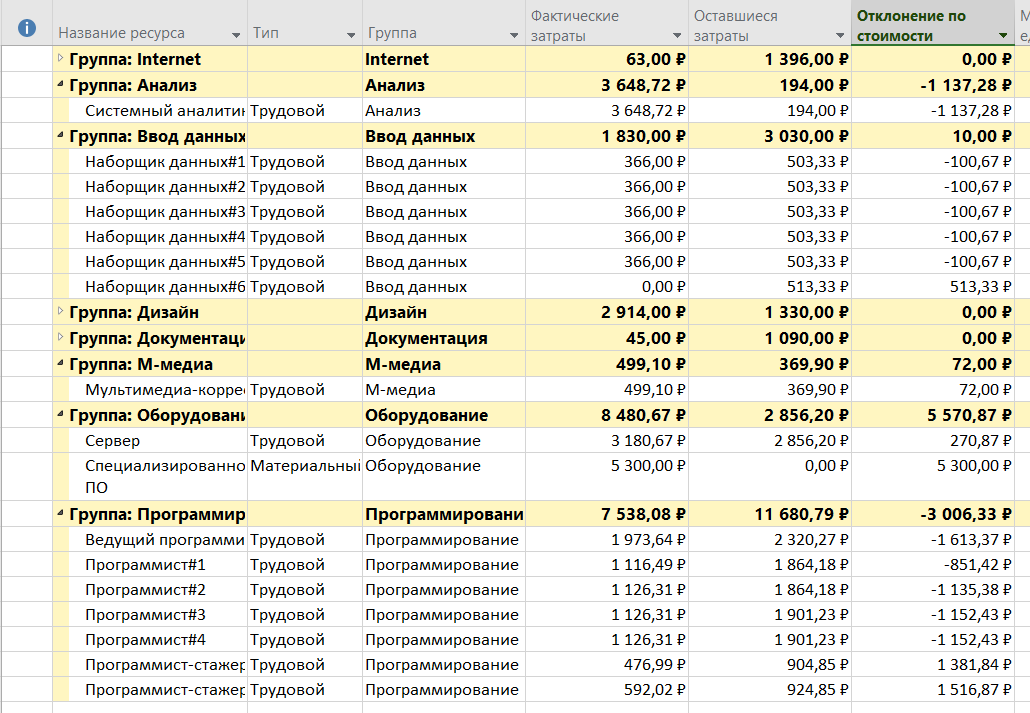
\includegraphics[scale=0.55]{inc/img/p_2.png}
	\end{center}
	\captionsetup{justification=centering}
	\label{fig:u3}
\end{figure}

\newpage

Анализ отклонений по стоимости прямых ресурсов:

\begin{enumerate}
    \item отклонение по стоимости группы ресурсов <<Анализ>> (-1137 руб) связано с уменьшением доступности системного аналитика до 70\%;
    \item отклонение по стоимости группы ресурсов <<Ввод данных>> (+10 руб) связано с наймом <<Наборщика данных 6>>;
    \item отклонение по стоимости группы ресурсов <<М-медиа>> (+72 руб) связано с увеличением зарплаты мультимедиа-корреспондента;
    \item отклонение по стоимости группы ресурсов <<Программирование>> (+3006 руб) связано с наймом двух новых программистов-стажеров;
\end{enumerate}


\newpage

\textbf{2. Используя таблицу освоенного объема, определите основные финансовые
показатели проекта на указанную дату отчета}

Таблица была открыта с помощью команд <<Вид → Таблицы → Другие таблицы → Освоенный объем>>.

\begin{figure}[h!]
	\begin{center}
		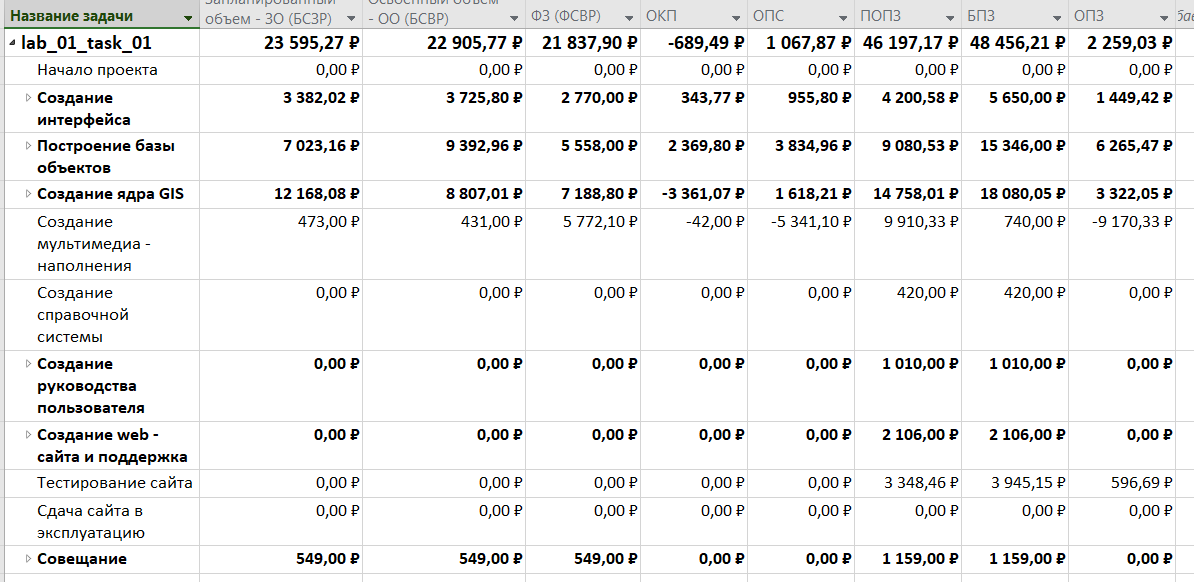
\includegraphics[scale=0.5]{inc/img/p_3.png}
	\end{center}
	\captionsetup{justification=centering}
	\label{fig:u3}
\end{figure}

Основные финансовые показатели:

\begin{itemize}
    \item[---] Запланированный объем (ЗО) – средства, которые были затрачены на
выполнение задачи в период с начала проекта до выбранной даты
отчета, если бы задача точно соответствовала графику и смете. Полученное значение: 23 595 рублей.
    \item[---] Освоенный объем (ОО) (БСВР) – это средства, которые были бы
затрачены на выполнение задачи с самого начала проекта до выбранной
даты отчета, если бы фактически выполненная работа оплачивалась
согласно смете. Полученное значение: 22 905 рублей.
    \item[---] Фактические затраты (ФЗ) (ФСВР) – средства, фактически
потраченные на задачи в период с начала проекта до выбранной даты
отчета. Полученное значение: 21 837 рублей.
    \item[---] Отклонение от календарного плана (ОКП) = БСВР – ЗО. Различие
между плановым и фактическим объёмом работы. Полученное значение: -689 рублей. Отрицательное значение свидетельствует об отставании проекта
(вызвано в уменьшением доступности аналитика до 70\%).
    \item[---] Отклонение по стоимости (ОПС) = БСВР – ФСВР. Сравнивает
сметную и фактическую стоимость выполненной работы и позволяет
выделить несоответствие сметы, вызванные разницей стоимости. Полученное значение: 1067 рублей. Положительное значение свидетельствует об имеющемся запасе
по смете (вызвано наймом программистов-стажеров и уменьшением затрат на задачи группы программирование).
    \item[---] Предварительная оценка по завершении (ПОПЗ) = ФСВР+ (Базовые
затраты-БСВР) / ИОС. Отображает ожидаемые общие затраты для
задачи, расчет которых основан на предположении, что оставшаяся
часть работы будет выполнена в точном соответствии со сметой. Полученное значение: 46 197 рублей.
    \item[---] Затраты по базовому плану (БПЗ) показывают фиксированные
затраты и стоимость ресурсов согласно базовому плану. Полученное значение: 48 456 рублей.
    \item[---] Отклонение по завершению (ОПЗ) – разность между БПЗ и ПОПЗ,
если эта величина отрицательна, то наблюдается перерасход средств. Полученное значение: 2 259 рублей. Положительное значение свидетельствует об экономии средств.
\end{itemize}

Таким образом, на 08.05.24 проект отстает от базового плана по календарю, но
также есть запасы по смете, а к концу проекта по смете ожидается, что проект
выйдет меньше на 2 259 рублей.

\newpage

\subsection*{Задание 2: Работа с отчетами проекта}

\textbf{1. Определите, в какой период времени руководитель проекта будет
испытывать наибольшую потребность в деньгах.}

Отчет был создан с помощью команд <<Отчет → Наглядные отчеты → Отчет о бюджетной стоимости>>.

\begin{figure}[h!]
	\begin{center}
		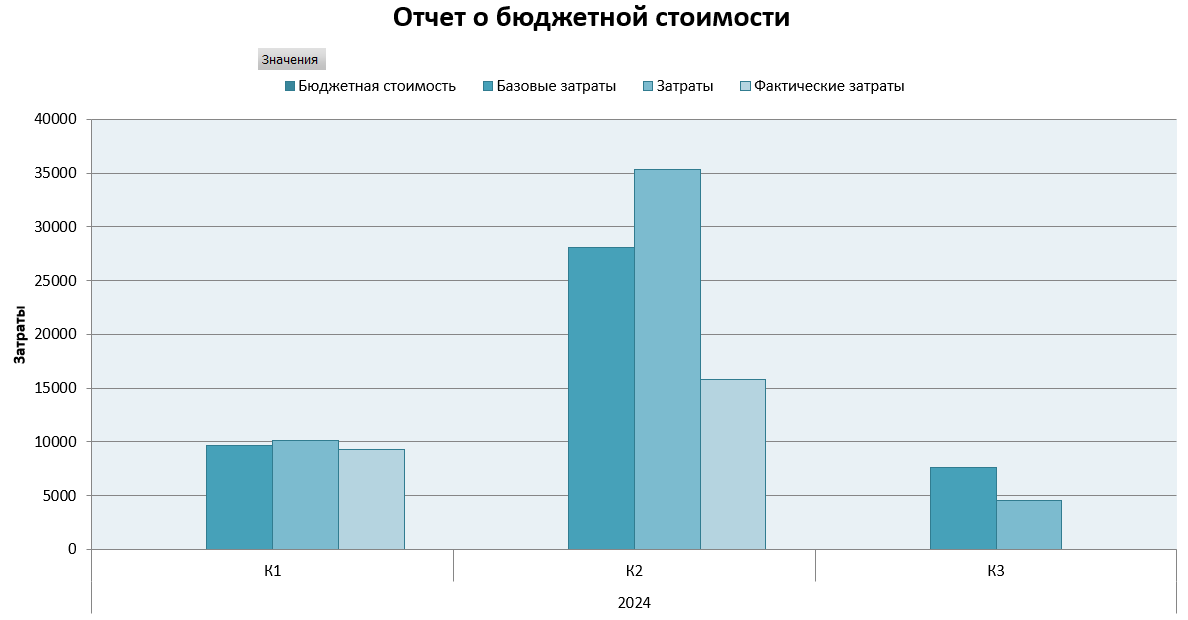
\includegraphics[scale=0.5]{inc/img/p_4.png}
	\end{center}
	\captionsetup{justification=centering}
	\label{fig:u3}
\end{figure}

\begin{figure}[h!]
	\begin{center}
		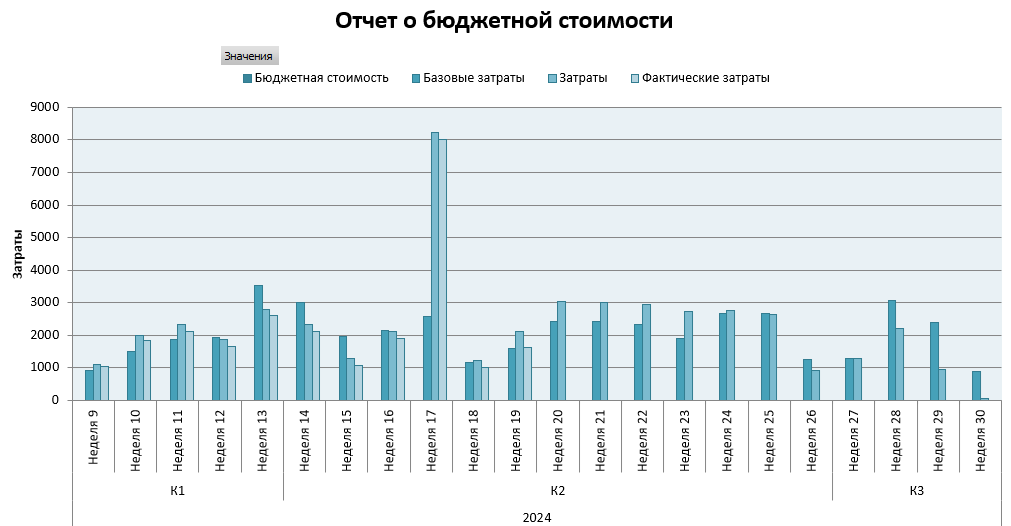
\includegraphics[scale=0.6]{inc/img/p_6.png}
	\end{center}
	\captionsetup{justification=centering}
	\label{fig:u3}
\end{figure}

\begin{figure}[h!]
	\begin{center}
		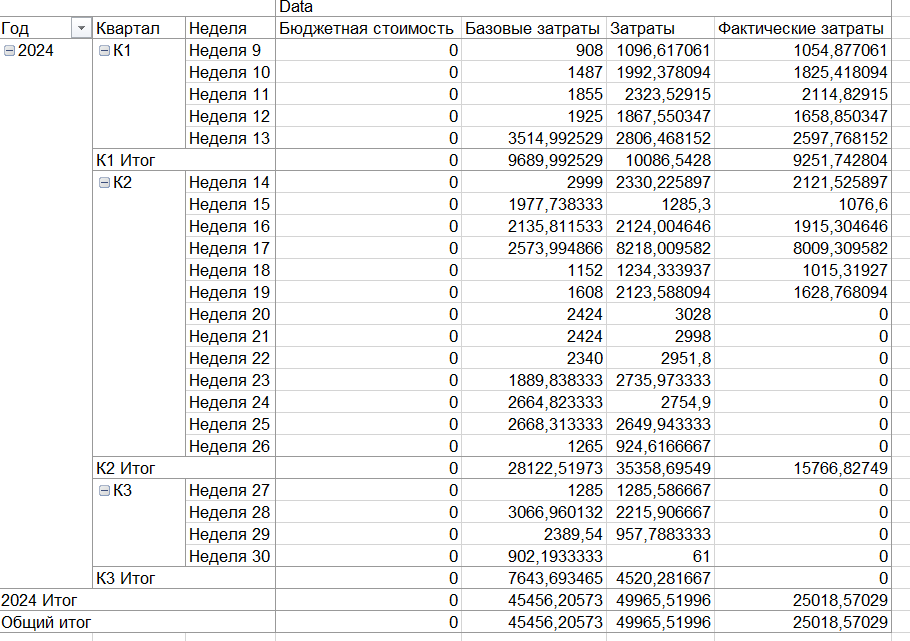
\includegraphics[scale=0.6]{inc/img/p_5.png}
	\end{center}
	\captionsetup{justification=centering}
	\label{fig:u3}
\end{figure}

\newpage

Отчет о бюджетной стоимости включает в себя следующие параметры:

\begin{itemize}
    \item[---] Базовые затраты --- это изначально запланированные затраты на выполнение задачи или проекта в целом. Их также называют затратами плана.
    \item[---] Затраты --- обычно под этим термином понимаются потенциальные или ожидаемые затраты на проект. Это может включать в себя текущие оценки расходов.
    \item[---] Фактические затраты --- это действительные затраты на проект. Они могут отражать стоимость работы, которая уже была выполнена.
\end{itemize}

Таким образом, наибольшую потребность в деньгах руководитель будет испытывать во втором квартале, или, если рассматривать более подробно, на 17 неделе. Это связано с перераспределением средств в задачах <<Программирование интерфейса>> и <<Наполнение базы объектов>> (найм новых сотрудников позволил уменьшить время выполнения задач, однако стоимость их на конкретную неделю возрасла).

\newpage

\textbf{2. Выведите на экран задачи, превышающие бюджетную стоимость}

Отчет о превыщении затрат был создан с помощью команд <<Отчет → Затраты → Превышение затрат>>.

\begin{figure}[h!]
	\begin{center}
		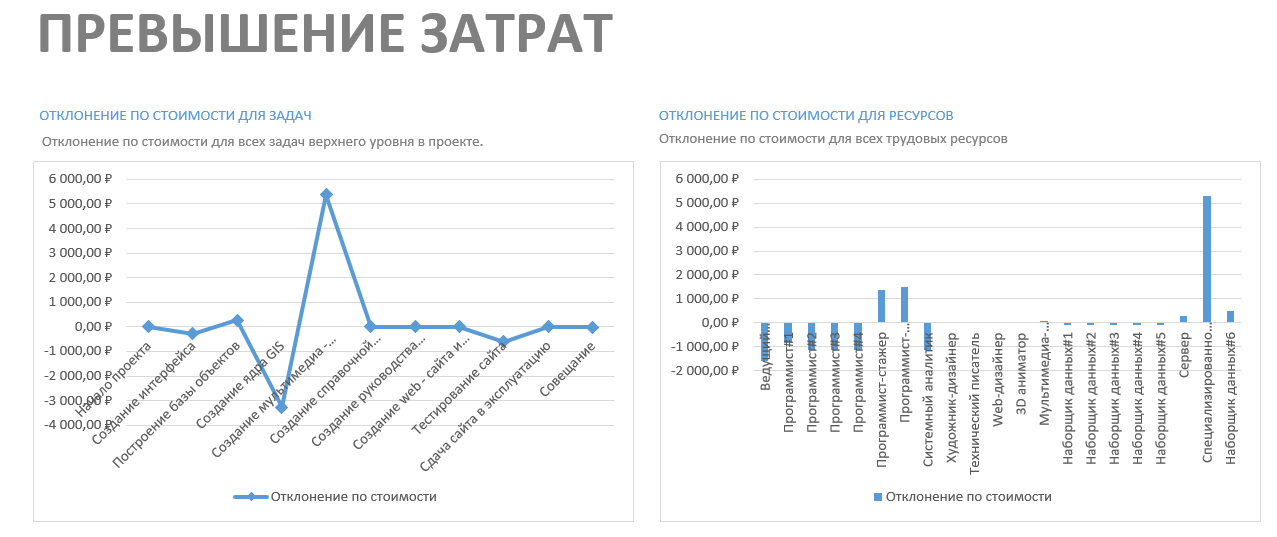
\includegraphics[scale=0.5]{inc/img/p_7.png}
	\end{center}
	\captionsetup{justification=centering}
	\label{fig:u3}
\end{figure}

\begin{figure}[h!]
	\begin{center}
		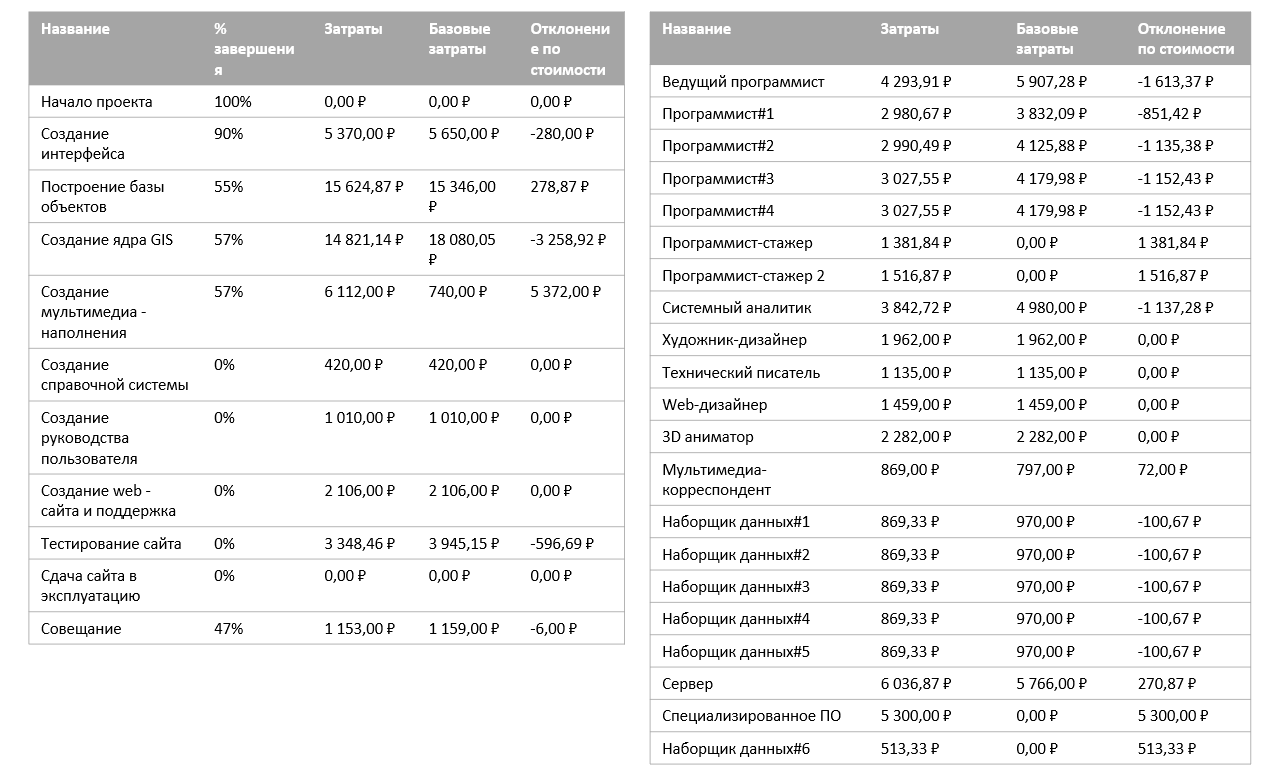
\includegraphics[scale=0.5]{inc/img/p_8.png}
	\end{center}
	\captionsetup{justification=centering}
	\label{fig:u3}
\end{figure}

Наиболее значительное превышение затрат ожидается в задаче создания мультимедиа наполнения. Отклонение вызвано увеличением заработной платы мультимедиа-корреспондента, а а также покупкой лицензии на специальное оборудование.

При этом в задаче создание ядра GIS ожидается
уменьшение затрат (в связи с наймом двух стажеров-разработчиков), которое частично скомпенсирует
упомянутые превышения.

\subsection*{Задание 3: Анализ вариантов декомпозиции работ в проекте}

\textbf{1. Предложите другой вариант декомпозиции работ проекта, приняв за
основу этапы каскадной модели жизненного цикла}

До (статистика из ЛР 2):
\begin{figure}[h!]
	\begin{center}
		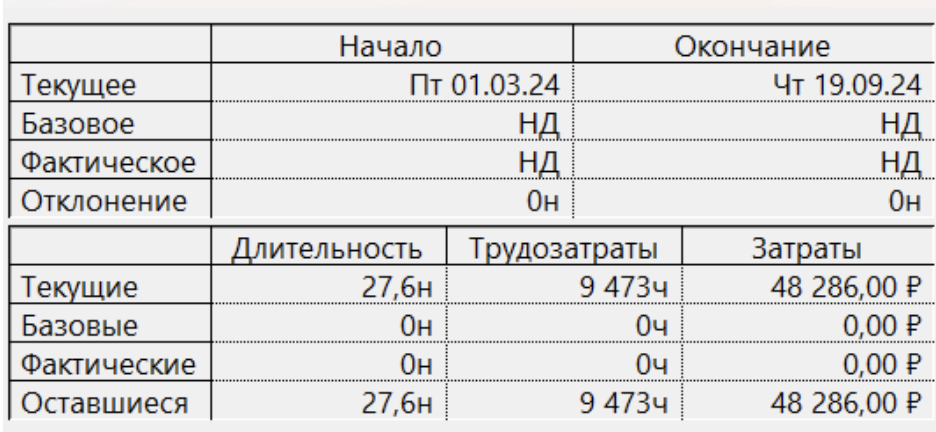
\includegraphics[scale=0.6]{inc/img/p_9.png}
	\end{center}
	\captionsetup{justification=centering}
	\label{fig:u3}
\end{figure}

\begin{figure}[h!]
	\begin{center}
		
\includegraphics[scale=0.55]{inc/img/p_10.png}
	\end{center}
	\captionsetup{justification=centering}
	\label{fig:u3}
\end{figure}

\begin{figure}[h!]
	\begin{center}
		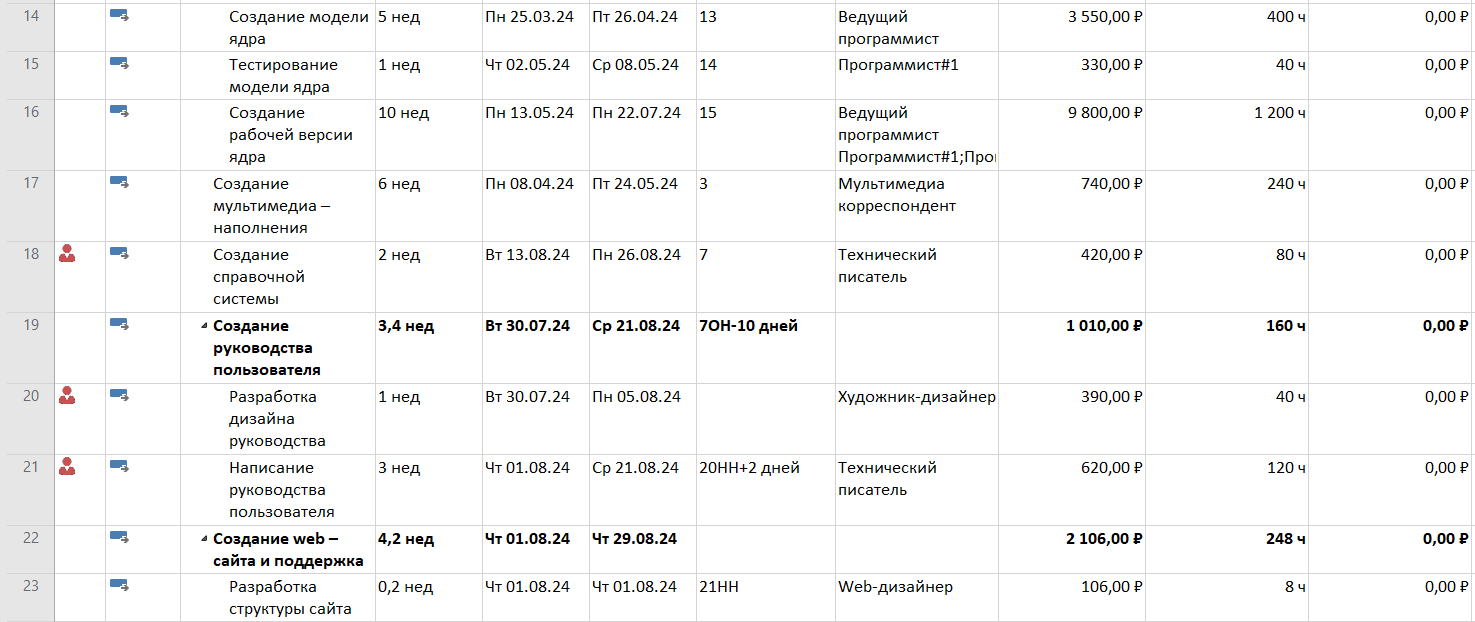
\includegraphics[scale=0.55]{inc/img/p_11.png}
	\end{center}
	\captionsetup{justification=centering}
	\label{fig:u3}
\end{figure}

\begin{figure}[h!]
	\begin{center}
		
\includegraphics[scale=0.5]{inc/img/p_12.png}
	\end{center}
	\captionsetup{justification=centering}
	\label{fig:u3}
\end{figure}

\newpage

Было 3 перегрузки из-за наложения задач:
\begin{itemize}
    \item[---] у системного аналитика из-за наложения задач «Анализ и построение структуры и базы объектов» и «Анализ и проектирование ядра»;
    \item[---] у художника-дизайнера из-за наложения задач «Разработка дизайна руководства» и «Разработка дизайна сайта»;
    \item[---] у технического писателя из-за наложения задач «Написание руководства пользователя» и «Создание справочной системы».
\end{itemize}

Была проведена декомпозиция с точки зрения каскадного подхода: на фазы анализ требований, проектирование, кодирование и тестирование.

\newpage

\begin{figure}[h!]
	\begin{center}
		
\includegraphics[scale=0.35]{inc/img/p_14.png}
	\end{center}
	\captionsetup{justification=centering}
	\label{fig:u3}
\end{figure}

\begin{figure}[h!]
	\begin{center}
		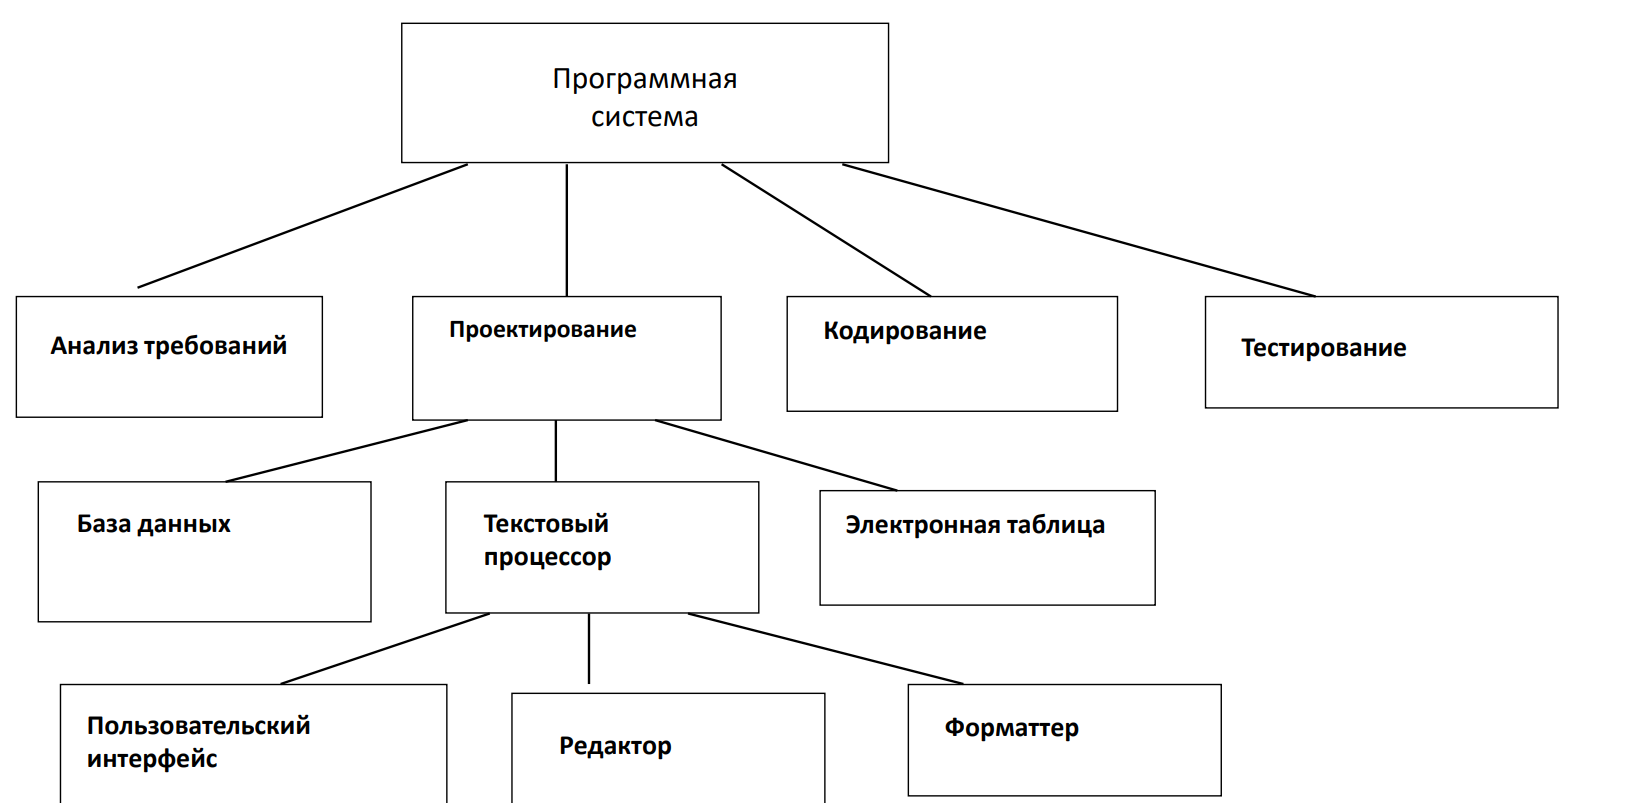
\includegraphics[scale=0.4]{inc/img/p_13.png}
	\end{center}
	\captionsetup{justification=centering}
	\label{fig:u3}
\end{figure}

\begin{itemize}
    \item[---] Исходные номера задач были оставлены в названиях для удобства.
    \item[---] Если для какой-то фазы были назначены фиксированные затраты, они переносились в одну из ее задач (исходя из здравого смысла). 
    \item[---] Если на всю фазу был назначен некоторый ресурс, он назначался отдельно на каждую из подзадач.
    \item[---] Последовательность (связи) внутри новых фаз была сохранена из первоначального проекта, между новыми фазами – последовательно от фазы к фазе.
    \item[---] Добавлена задача «Анализ требований» продолжительностью в 1 неделю.
\end{itemize}

После:

\begin{figure}[h!]
	\begin{center}
		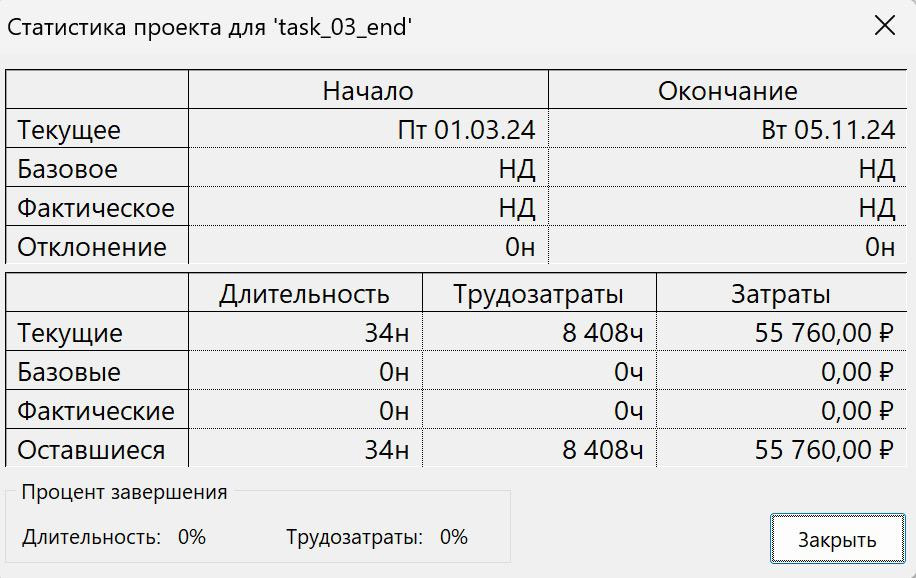
\includegraphics[scale=0.35]{inc/img/p_16.jpg}
	\end{center}
	\captionsetup{justification=centering}
	\label{fig:u3}
\end{figure}

Затраты и длительность проекта возросли, однако стоит понимать, что эти данные некорректны, потому что не было проведено выравнивание ресурсов, в следствие которого, длительность проекта бы возросла, а затраты значительно снизились, потому что не пришлось бы платить сотрудникам сверхурочную ставку за рабочие часы.

\begin{figure}[h!]
	\begin{center}
		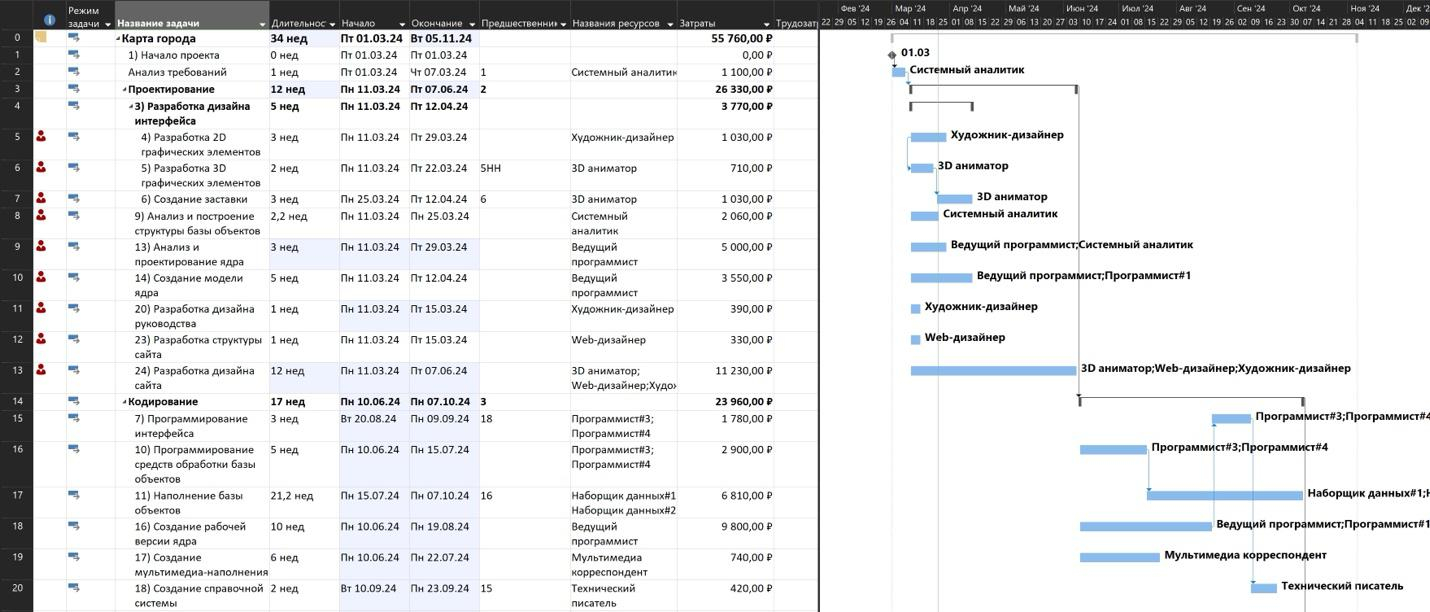
\includegraphics[scale=0.3]{inc/img/p_17.jpg}
	\end{center}
	\captionsetup{justification=centering}
	\label{fig:u3}
\end{figure}


\begin{figure}[h!]
	\begin{center}
		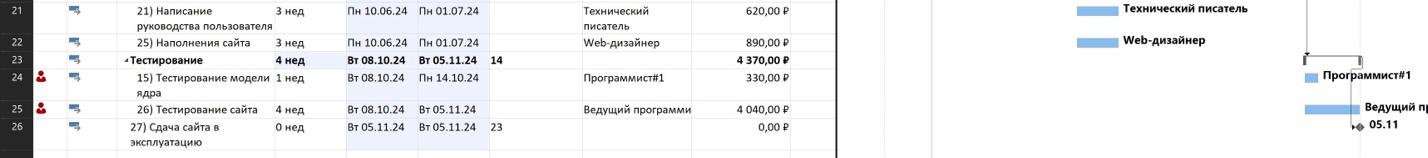
\includegraphics[scale=0.3]{inc/img/p_18.jpg}
	\end{center}
	\captionsetup{justification=centering}
	\label{fig:u3}
\end{figure}

\begin{figure}[h!]
	\begin{center}
		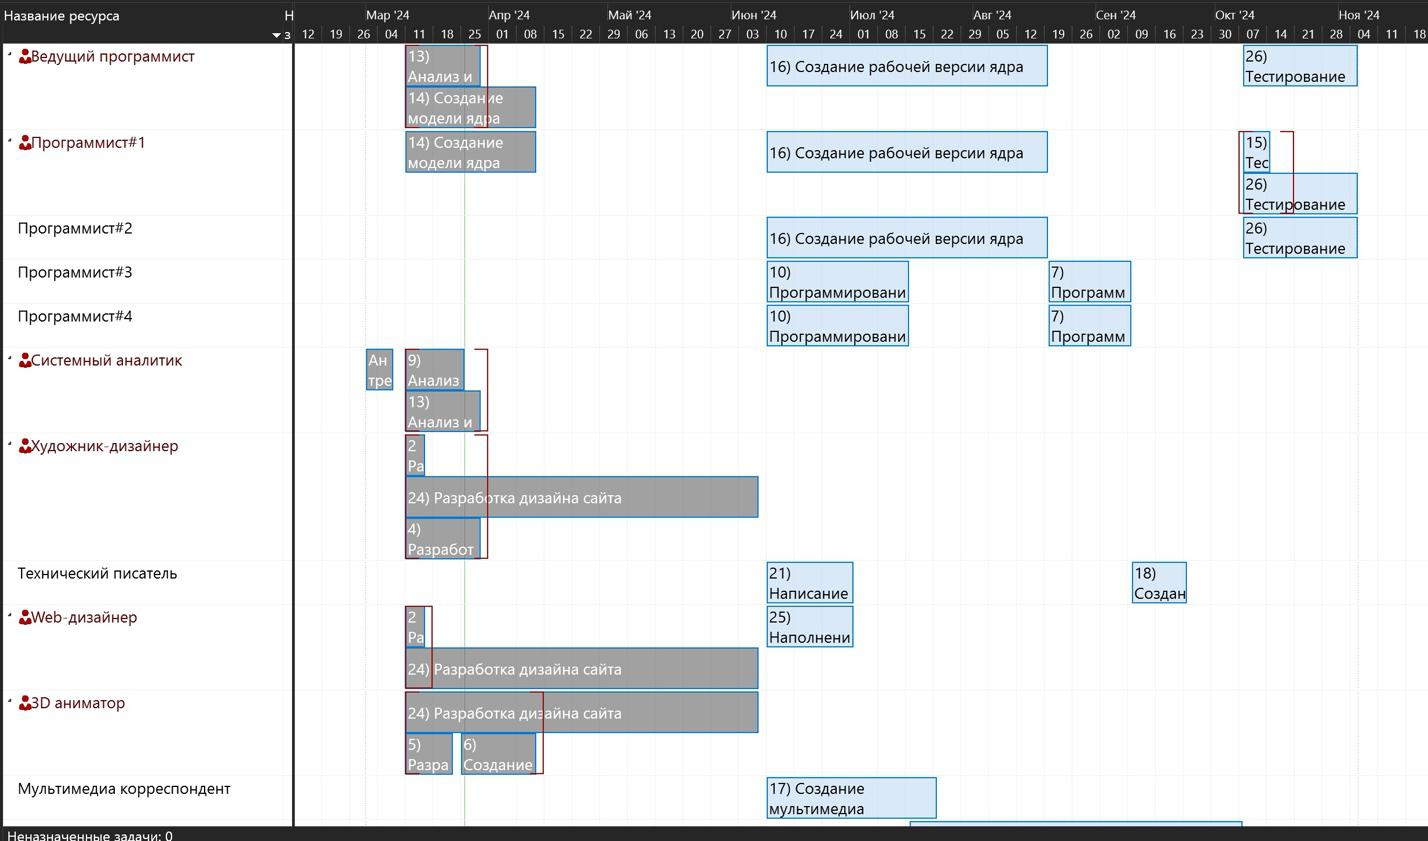
\includegraphics[scale=0.3]{inc/img/p_19.jpg}
	\end{center}
	\captionsetup{justification=centering}
	\label{fig:u3}
\end{figure}

\newpage

По итогу реализации каскадного подхода было получено большое количество перегрузок, в результате устранения которых длительность проекта бы увеличилась, а стоимость не изменилась. 

Основной проблемой каскадного подхода является простой ресурсов в то время, пока выполняются стадии проекта, на которых они не задействованы.

\subsection*{Вывод}

Была проведена работа с таблицей освоенного объёма, проанализированы траты по кварталам.

Была проведена декомпозиция задач с использованием каскадного подхода. 

Выявлены недостатки и преимущества каскадного подхода по сравнению с традиционной декомпозицией работ, привязанной к структуре продукта:

\begin{enumerate}
    \item при каскадном подходе задачи делятся на фазы так, что сотрудники с определенными компетенциями задействованы в этих отдельных фазах. Это вызывает перегрузки ресурсов, которые требуется устранять. 
    \item в каскадной декомпозиции задач сложно рассмотреть, когда определенная часть продукта будет завершена: когда будут собраны данные, когда готово ядро, а когда – сайт. 
    \item в каскадной декомпозиции есть «простои», а анализ критического пути не дает возможности увидеть варианты решения проблемы.
    \item традиционные декомпозиции детализируются и планируются либо слишком подробно, либо недостаточно подробно.
    \item традиционные декомпозиции работ специфичны для каждого проекта, поэтому сравнение разных проектов обычно оказывается затруднительным или невозможным.
\end{enumerate}

Сравнение с лабораторной работой 2.

ЛР 2:

\begin{figure}[h!]
	\begin{center}
		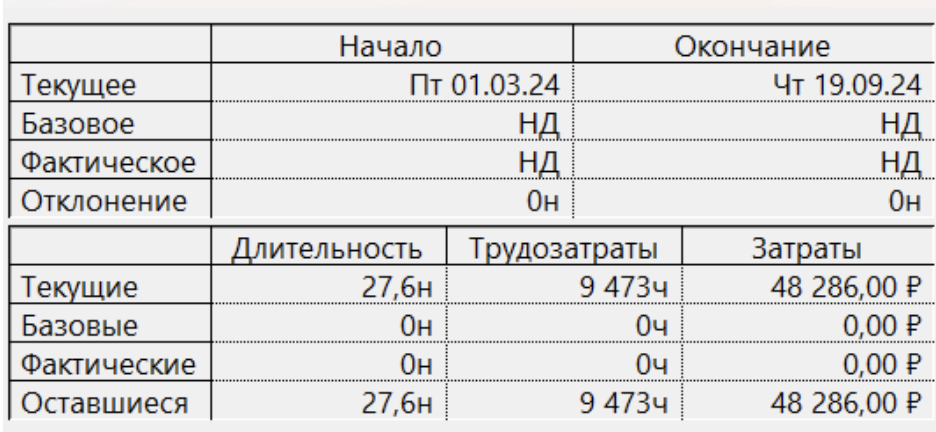
\includegraphics[scale=0.6]{inc/img/p_9.png}
	\end{center}
	\captionsetup{justification=centering}
	\label{fig:u3}
\end{figure}

ЛР 5:

\begin{figure}[h!]
	\begin{center}
		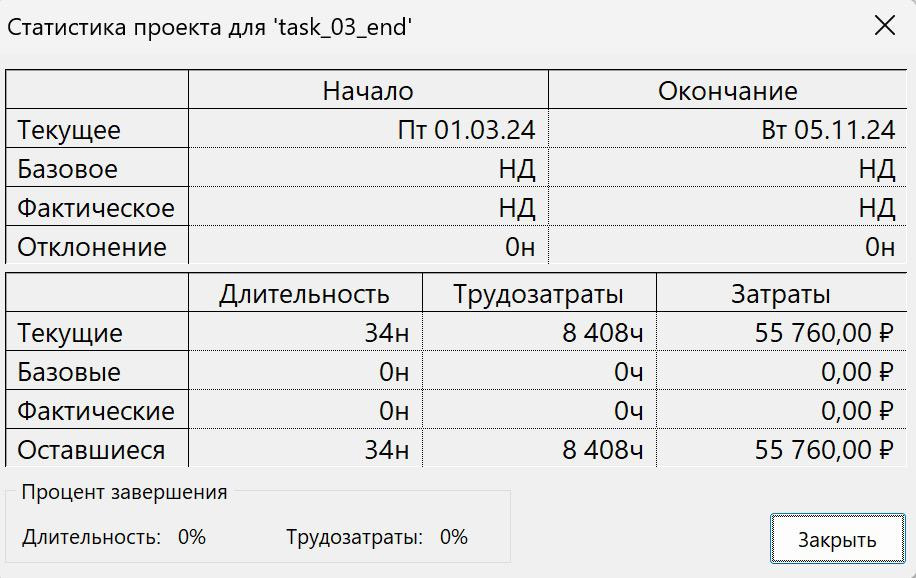
\includegraphics[scale=0.35]{inc/img/p_16.jpg}
	\end{center}
	\captionsetup{justification=centering}
	\label{fig:u3}
\end{figure}

При этом, стоит понимать, что данные приведены без устранения перегрузок, и в результате их устранения длительность бы значительно увеличилась.